%\flushleft

\begin{table}[!h]
  \caption{List of user stories}
  \centering
  \begin{tabular}{l||l|l|l|l|}
    ID & Name & Size &  Source & Sprint\\
    \hline
    R1&Research Apriori&Medium&Project brief&1\\
    R2&Research StAX Parser&Small&Project brief&1\\
    1&Testing&Medium&Project brief&5\\
    2&Imports in tree structure&Medium&Client&2\\ %Original ID was 2.001; 
    3&Testrun chart&Medium&Project brief&3\\
    7&Testrun table&Medium&Project brief&2\\
    8&Association Analysis&Large&Project brief&3\\
    9&Testrun Selection&Medium&Project brief&2\\
    12&Store XML in classes&Medium&Assumed by us&1\\ 
    18&XMLParsing&Medium&Project brief&1\\
    21&Documentation&Large&Engineering practice&2\\
    23&Implement Apriori Algorithm&Large&Project brief&4\\
    24&Display Analysis Data&Medium&Project brief&4\\
    25&Additional usage scenario&Medium&Project brief&5\\
    26&Code Documentation&Small&Project brief&5\\
    27&Distribution with suited license&Small&Project brief&5\\ %not sure about origin of 27/28
    28&Creating a help function&Small&Project brief&5\\
    213&Evolution of a class&Large&Assumed by us&4\label{evolution213}\\ 
  
	\end{tabular}
  \label{tab:user_stories}
\end{table}

As you may notice our user stories have quite strange IDs with a lot of numbers missing in between. This is because in the beginning we wanted to prevent that the IDs indicate an order. Retrospectively, we came to the conclusion that this was a mistake, as it caused more confusion in our group.\\
In the end we tried to fix this a little bit (user stories 23-28), however, the project was already quite far in progress, so the majority of user stories still has random IDs.  \\
\newline
In Sprint 0 we discussed the content of the project brief and to make sure we all were on the same page we proceeded to draw a first use case diagram. This was helpful in multiple ways, as it gave us an overview over the whole project in addition to helping us figure out functional requirements.\\
The use case diagram was always maintained when we received new requirements from the client or we changed our code in such way that we had to update the diagram. Thanks to this progress, we for example came to the conclusion that a start screen where you can select xml-files makes a lot of sense, since all features depend on data, which has to be parsed first.\\
Another source of requirements is the feedback we received from the client to our paper prototypes we engineered together. These were very important, since it allowed us to work confidently on the GUI. %They were truly great. He loved them. Tremendous. ANYONE WHO SAIS OTHERWISE IS FAKE NEWS. SAD.

\begin{sidewaysfigure}
	\begin{center}
		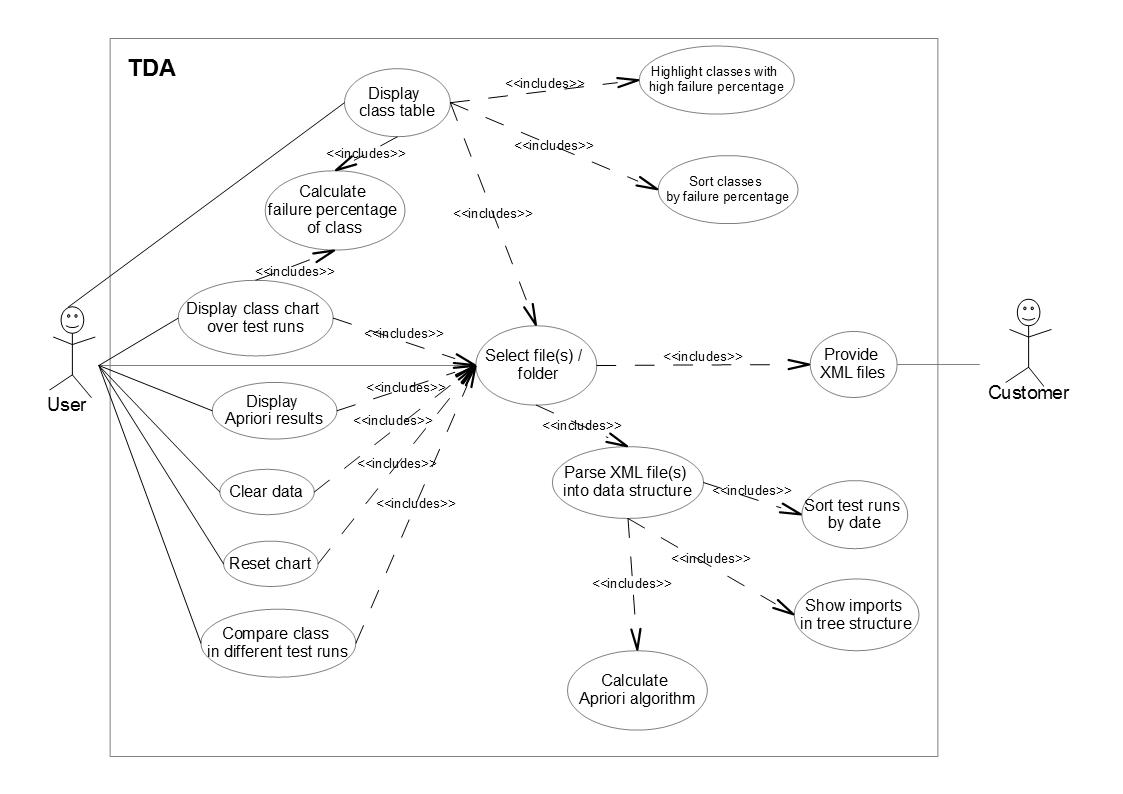
\includegraphics[scale=0.6]{pics/UseCaseDiagram.jpg}
		\caption{Use case diagram}
		\label{use-case}
	\end{center}	
\end{sidewaysfigure}
Based on this use case diagram \ref{use-case} we then proceeded to write user stories and corresponding tasks. This way we always had the requirements in eye-sight on the task-board.

\subsection{Requirements derived from project brief}
\subsubsection{Functional requirements}
\begin{itemize}	
	\item A table shall show all tested classes of one testrun\\
	Fit criteria: testruns ordered descending by failure percentage and highlight red if failure percentage is higher than 75\% and yellow if it's between 50 and 75\% 
	\item A chart shall display the change of a specific class over all parsed testruns\\
	Fit criteria: every class can be added to chart only once - not multiple times; Is good readable even with a lot of testruns
	\item Association analysis shall use the well-established Apriori algorithm\\
	Fit criteria: Strong rules are generated from frequent item sets
	\item XML-files shall be parsed using the StAX parser\\
	Fit criteria: Every correct xml-file will be read and stored in our data structure
	\item The user shall be able to select a specific testrun to get more information\\
	Fit criteria: When testrun is selected the table and all relevant testrun details will be shown.
	\item The association analysis output shall be displayed in a convenient way.\\
	Fit criteria: It visualizes the output in an easy, but contentful way, which is approved by the client.
	\item Two more usage scenarios shall be suggested to the client and implemented\\
	Fit criteria: Scenarios are accepted by the client and implemented to his wishes
	\item The software shall be distributed with a suited open-source licence\\
	Fit criteria: Licence shall be visible from within the software and be free("libre")
	\item A manual shall be accessible from within the software\\
	Fit criteria: Explains all features and how they are used
\end{itemize}

\subsubsection{Non-Functional requirements}
\begin{itemize}
	\item All features shall be tested sufficiently\\
	Fit criteria: Coverage of at least 90\%
	\item Source code shall be documented properly\\
	Fit criteria: Every class is documented according to the project brief
\end{itemize}

\subsubsection{Development constraints}
\begin{itemize}
	\item The software has to run on a standard SWT-lab PC
	\item Software shall be implemented in Java; documented using Jdoc; tested with JUnit;
	\item Copied code shall be cited with its source
	\item Development shall be done via the SWT-Git-repository
	\item Commit messages shall have the following format: \\
	SPRINT n SUBSTANTIAL m \\
	documentation of commit \\
	full name of responsible person
	\item The file structure shall be as follows:
	\begin{itemize}
		\item 'src' containing source files
		\item 'test' containing JUnit tests
		\item 'doc' containing JavaDoc of the sources
		\item 'uml' containing UML-diagram files
	\end{itemize}
	\item Final release shall look as follows:
	\begin{itemize}
		\item source files; unit tests; Jdoc
		\item binary release (jar)
		\item project report
	\end{itemize}
	
\end{itemize}
\subsection{Requirements assumed by us}
\subsubsection{Functional requirements}
\begin{itemize}
	\item The class overview in the sidebar shall display all classes in a tree structure\\
	Fit criteria: classes are in a tree based on packet structure and clicking on them inserts them in the chart
	\item All relevant data from the xml-files shall be stored in corresponding classes(data structure)\\
	Fit criteria: all unit tests on the data structure pass
	\item The user shall be able to compare two specific testruns of one class with respect to its unit tests.\\
	Fit criteria: Not possible to compare different classes; Shows all passed and failed unit tests and the difference between two runs
\end{itemize}

\subsubsection{Non-functional requirements}
\begin{itemize}
	\item The software shall run reliably\\
	Fit criteria: Shall maintain a 95\%+ uptime
	\item Parsing and computing shall be reasonable fast with respect to the amount of files parsed\\
	Fit criteria: Should not take longer than 2 minutes for 1000 files
	\item The parser shall only parse xml-files with the correct format\\
	Fit criteria: When a wrong format is detected an exception shall be thrown
\end{itemize}
\subsection{Requirements added by client}
\subsubsection{Functional requirements}

\begin{itemize}

%Sprint 1:
\item choose a folder and parse all containing XML files in the folder and its subdirectory\\
Fit criteria: every *.xml file is parsed and added to the data structure

%Sprint 2:
%Maybe NFR:
\item Table: classes with failure percentages between 50 - 75\% should be highlighted yellow and failure percentages between 75 - 100\% should be highlighted red; it should be possible to hide/show all classes with a failure percentage of 0\%\\
Fit criteria: The table highlights the classes correctly according to failure percentage
\item Failure percentages in table should be rounded to 2 decimals\\
Fit criteria: All percentages are rounded correctly
\item Testrun totals: a note, stating that not all totals of the testrun are shown above the table should be visible; a button shall enable the user to see all totals\\
Fit criteria: All relevant information is displayed, when the details button is pressed

%Sprint 3:
\item one click in tree sidebars for selecting files (no doubleclick)\\
Fit criteria: Only one click is needed to select testruns or classes
\item hover over chart entries shall show testrun information\\
Fit criteria: On hover the start time and the number of failed/passed unit tests shall be displayed
\item chart shall have its own page instead of being shown in the main window below the class table\\
Fit criteria: the chart shall not be under the table anymore, so it has more space to display data
\item The functions to filter the Apriori results by confidence and distance should be implemented\\
Fit criteria: Correct filtering of confidence and by distance shall be possible

\item A second additional usage scenario should be proposed, but due to the given point in time the focus should be to finalize the already implemented functionality\\
Fit criteria: The scenario is presented to the client and accepted


Fit criteria: 

\end{itemize}

\subsubsection{Non-functional requirements}
\begin{itemize}
%Sprint 2:
\item The software shall load most of its data in the beginning, so you can use the tool without waiting times later on\\
Fit criteria: When switching between features there shall be minimal loading times if at all



\item program shall adapt its layout automatically to lower resolutions or resizing\\
Fit criteria: The content is always well readable, no matter the resolution or display size
%Sprint 4:
%NFR
\item The outcome of the Apriori algorithm should be visualized in a better way, since the two tables are not easy to read.\\
Fit criteria: A easier to understand visualization shall make clear what classes are dependent
\end{itemize}